\documentclass[a4paper, 12pt, english]{article}

% \usepackage[portuges]{babel}
\usepackage[utf8]{inputenc}
\usepackage{amsmath,amssymb}
\usepackage{graphicx}
\usepackage{subfig}
\usepackage[colorinlistoftodos]{todonotes}

\usepackage{indentfirst}
\usepackage{verbatim}
\usepackage{textcomp}
\usepackage{gensymb}
\usepackage{float}
\usepackage{multirow}
\usepackage{pgfplots}
\pgfplotsset{compat=1.17}

\usepackage{relsize}

\usepackage{lipsum}% http://ctan.org/pkg/lipsum
\usepackage{xcolor}% http://ctan.org/pkg/xcolor
\usepackage{xparse}% http://ctan.org/pkg/xparse
\NewDocumentCommand{\myrule}{O{1pt} O{2pt} O{black}}{%
	\par\nobreak % don't break a page here
	\kern\the\prevdepth % don't take into account the depth of the preceding line
	\kern#2 % space before the rule
	{\color{#3}\hrule height #1 width\hsize} % the rule
	\kern#2 % space after the rule
	\nointerlineskip % no additional space after the rule
}
\usepackage[section]{placeins}

\usepackage{booktabs}
\usepackage{colortbl}%
\newcommand{\myrowcolour}{\rowcolor[gray]{0.925}}

\usepackage[obeyspaces]{url}
\usepackage{etoolbox}
\usepackage[colorlinks,citecolor=black,urlcolor=blue,bookmarks=false,hypertexnames=true]{hyperref}

\usepackage{geometry}
\geometry{
	paper=a4paper, % Change to letterpaper for US letter
	inner=3cm, % Inner margin
	outer=3cm, % Outer margin
	bindingoffset=.5cm, % Binding offset
	top=2cm, % Top margin
	bottom=2cm, % Bottom margin
	%showframe, % Uncomment to show how the type block is set on the page
}
\usepackage{fancyhdr}

% Define header and footer
\pagestyle{fancy}
\fancyhf{}
\lhead{ENER 104L}
\rhead{iSciM, Habib University} % Right-aligned page number in the header
\rfoot{\thepage} % Right footer text
%*******************************************************************************%
%************************************START**************************************%
%*******************************************************************************%
\begin{document}

%************************************TITLE PAGE**************************************%
\begin{titlepage}
	\begin{center}
		\textbf{\LARGE Habib University}\\[0.5cm]
		\textbf{\large iSciM}\\[0.2cm]
		\textbf {\large Fall 2023}\\[0.2cm]
		\vspace{20pt}
		\includegraphics[width=5cm]{../habiblogo.jpg}\\[1cm]
		\par
		\vspace{20pt}
		\textbf{\Large ENER 104L RENEWABLE ENERGY}\\
		\vspace{15pt}
		\myrule[1pt][7pt]
		\textbf{\LARGE  LABORATORY REPORT 8}\\
		\vspace{15pt}
		\textbf{\large Electrical Energy from Wind Energy}\\
		\myrule[1pt][7pt]
		\vspace{25pt}
		\begin{tabular}{@{}p{5cm}p{3cm}@{}}
			\textbf{\large Student Name} & \textbf{\large Student ID} \\
			Ali Asghar Yousuf            & ay06993                    \\ % No1 
			Syed Ibrahim Ali Haider      & sh06565                    \\ % No2
		\end{tabular}

		\vspace{10pt}
		\begin{tabular}{@{}p{5cm}p{3cm}@{}}
			\textbf{\large Group Name} & \textbf{\large Group No.} \\
			Insane Fr                  & 1                         \\
		\end{tabular}

		\vspace{45pt}
		\textbf {\large Lab Instructors:}\\[0.2cm]
		\Large {Paishwa Naqvi}\\[0.1cm]
		\Large {Mah Noor Jamil}\\[0.1cm]
		\Large {Amber Talat}\\[0.1cm]
	\end{center}

	\par
	\vfill
	\begin{center}
		\textbf{\today}\\
	\end{center}

\end{titlepage}

%************************************TABLE OF CONTENTS**************************************%

%  %Sumário
%  \newpage
%  \tableofcontents
%  \thispagestyle{empty}
%  %End Sumário

%********************************%
%***********SECTION 1************%
%********************************%
\newpage
\section{Objectives}
\begin{itemize}
	\item To understand the working principle of a wind turbine to generate electricity.
	\item To understand the impact of wind speed and direction on the power output of a
	      wind turbine.
	\item To understand the advantages and disadvantages of wind energy as a renewable
	      energy source.
\end{itemize}

\section{Abstract}
Wind energy is a renewable energy source that is generated by the movement of
air masses in the atmosphere. Wind energy is a clean source of energy that does
not contribute to global warming. Wind energy is also a very cost-effective
source of energy. Wind energy is harnessed by wind turbines that convert the
kinetic energy of the wind into electrical energy. Wind turbines are usually
installed in areas with high wind speeds. In this lab, we will be using a small
wind turbine to understand the working principle of a wind turbine and to
understand the impact of wind speed and direction on the power output of a wind
turbine.

\section{Result and Analysis}
\subsection{Part A}
In this part of the experiment, we used a blower and a small wind turbine to
understand the working principle of a wind turbine. We were supposed to use a
light bulb to measure the power output of the wind turbine. However, due to
some technical difficulties, we were unable to use the light bulb. We used a
multimeter to measure the current output of the wind turbine. We used the
multimeter to measure the current output of the wind turbine at different
supply voltages.

\subsubsection{Experiment 1}
The distance between the blower and the wind turbine was kept constant at 5 cm
for all the supply voltages. The current output of the wind turbine was
measured at supply voltages of 6 V, 8 V, 10 V, and 12 V. The current output of
the wind turbine was found to be 0.01 mA for all the supply voltages.

\begin{table}[H]
	\centering
	\caption{Current Table for Experiment 1}
	\label{tab:table1}
	\begin{tabular}{@{}ll@{}}
		\toprule
		\textbf{Supply Voltage (V)} & \textbf{Current (mA)} \\ \midrule
		6                           & 0.01                  \\
		8                           & 0.01                  \\
		10                          & 0.01                  \\
		12                          & 0.01                  \\ \bottomrule
	\end{tabular}
\end{table}

\subsubsection{Experiment 2}
In this experiment, the distance between the blower and the wind turbine was
kept the same at 5 cm. However, we placed our hand in front of the blower to
obstruct the flow of air. The current output of the wind turbine was measured
at supply voltages of 6 V, 8 V, 10 V, and 12 V. The current output of the wind
turbine was found to be 0.00 mA for all the supply voltages.

\begin{table}[H]
	\centering
	\caption{Current Table for Experiment 2}
	\label{tab:table2}
	\begin{tabular}{@{}ll@{}}
		\toprule
		\textbf{Supply Voltage (V)} & \textbf{Current (mA)} \\ \midrule
		6                           & 0.00                  \\
		8                           & 0.00                  \\
		10                          & 0.00                  \\
		12                          & 0.00                  \\ \bottomrule
	\end{tabular}
\end{table}

\subsection{Part B}
In this part of the experiment, we varied the distance between the blower and
the wind turbine to understand the impact of wind speed and direction on the
power output of a wind turbine. We used a multimeter to measure the voltage
output of the wind turbine at different distances for different supply
voltages.

\begin{table}[H]
	\centering
	\caption{Voltage Readings at Different Distances for Various Supply Voltages}
	\label{tab:table3}
	\begin{tabular}{@{}cccccccc@{}}
		\toprule
		 &    & \multicolumn{4}{c}{\textbf{Supply Voltage (V)}}                    \\ \cmidrule(l){3-6}
		 &    & 12 V                                            & 10 V & 8 V & 6 V \\ \midrule
		\multirow{6}{*}{\rotatebox[origin=c]{90}{\textbf{Distance (cm)}}}
		 & 5  & 5.7                                             & 5.3  & 5.0 & 4.9 \\
		 & 10 & 5.2                                             & 4.5  & 4.5 & 4.3 \\
		 & 15 & 4.6                                             & 4.1  & 3.9 & 3.7 \\
		 & 20 & 3.9                                             & 3.3  & 3.1 & 3.0 \\
		 & 25 & 3.6                                             & 2.8  & 2.5 & 2.3 \\
		 & 30 & -                                               & -    & -   & -   \\ \bottomrule
	\end{tabular}
\end{table}

We plotted a graph of voltage output of the wind turbine against the distance
between the blower and the wind turbine for different supply voltages. The
graph is shown below. We were unable to measure the voltage output of the wind
turbine at a distance of 30 cm as the wind from the blower scattered so much
that the fan blade of the wind turbine kept on falling off due to wobbling.

$V_s$ represents the supply voltage of the blower.
\begin{figure}[H]
	\centering
	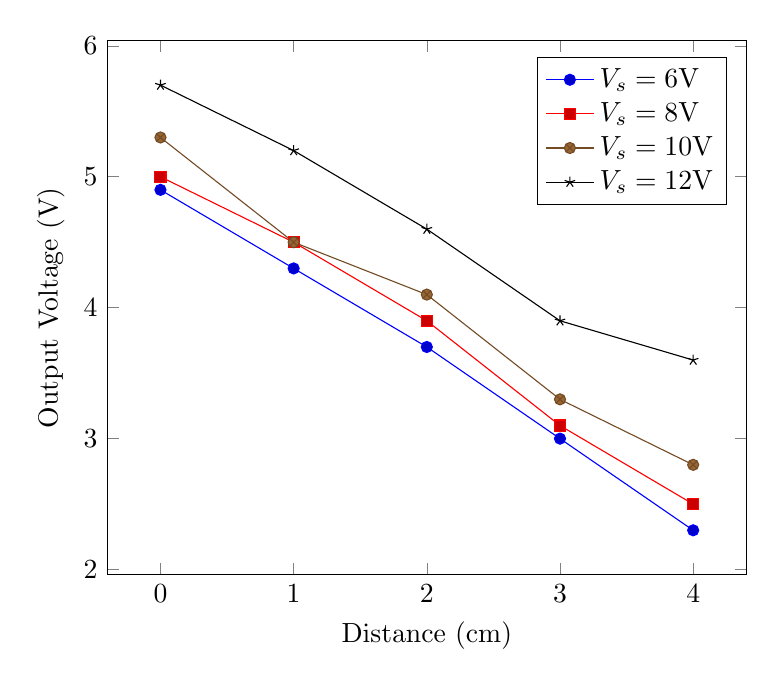
\begin{tikzpicture}
		\begin{axis}[
				width=0.8\textwidth,
				xlabel=Distance (cm),
				ylabel=Output Voltage (V),
				legend pos=north east,
				legend cell align={left},
				% enlarge x limits=0.15,
			]

			\addplot table[x expr=\coordindex, y=V6] {
					Distance V6
					5		4.9
					10		4.3
					15		3.7
					20		3.0
					25		2.3
				};
			\addlegendentry{$V_s = 6$V}

			\addplot table[x expr=\coordindex, y=V8] {
					Distance V8
					5		5.0
					10		4.5
					15		3.9
					20		3.1
					25		2.5
				};
			\addlegendentry{$V_s = 8$V}

			\addplot table[x expr=\coordindex, y=V10] {
					Distance V10
					5		5.3
					10		4.5
					15		4.1
					20		3.3
					25		2.8
				};
			\addlegendentry{$V_s = 10$V}

			\addplot table[x expr=\coordindex, y=V12] {
					Distance V12
					5		5.7
					10		5.2
					15		4.6
					20		3.9
					25		3.6
				};
			\addlegendentry{$V_s = 12$V}
		\end{axis}
	\end{tikzpicture}
	\caption{Voltage Output of the Wind Turbine Against the Distance Between the Blower and the Wind Turbine for Different Supply Voltages}
\end{figure}

We can see from the graph that the voltage output of the wind turbine decreases
as the distance between the blower and the wind turbine increases. This is
because the wind spreads out as it travels from the blower to the wind turbine
losing its kinetic energy. The wind turbine is able to harness less kinetic
energy from the wind as the distance between the blower and the wind turbine
increases. This results in a decrease in the voltage output of the wind
turbine.

Similarly, we can see from the graph that the output voltage of the wind
turbine decreases as the supply voltage decreases. This is because the wind
speed decreases as the supply voltage decreases. The wind turbine is able to
harness less kinetic energy from the wind as the supply voltage decreases. This
results in a decrease in the voltage output of the wind turbine.

\section{Conclusion}
In this lab, we used a blower and a small wind turbine to understand the
working principle of a wind turbine. Despite some technical difficulties, we
were able to achieve the objectives of the lab. We observed that the power
output of the wind turbine is directly proportional to the wind speed which
means that harnessing wind energy is not suitable for areas with low wind
speeds. We also observed that the power output of the wind turbine is directly
proportional to the wind direction which means that the positioning of the wind
turbine is very important. Nonetheless, wind energy is a very cost-effective
source of energy that does not require any fuel and does not contribute to
global warming.

\end{document}